% Santos. Include from a document with amsmath, graphicx, booktabs and float.
\subsection{Compensated electron density gradients at fixed deuterium gradient}\label{sec:additional-compensated}
The electrostatic kinetic electron--deuterium--helium model has reference densities $(n_e,n_D,n_{\rm He})=(1,0.75,0.125)$ and charges $(-1,+1,+2)$ with $\sum_s Z_s n_s=0$. The local density gradient condition $\sum_s Z_s n_s\omega_{n,s}=0$ gives $\omega_{n,\rm He}=4\omega_{n,e}-3$ at $\omega_{n,D}=1$. Helium's gradient changes with the electron gradient. GENE retained the negative helium gradient at the low endpoint.

We used proton-reference mass units with masses $(0.00054462,2,4)$, unit species temperature ratios and $\omega_T=2$ for each species. The common settings were $k_y\rho_{\rm ref}=0.7$, $\beta=0$, Landau \texttt{coll=0.01} and the original dipole geometry. The main scan used IV, automatic stepping and $24/48/24$. The two-species control at $\omega_{n,e}=\omega_{n,D}=1$ has a different composition and is shown separately. At electron gradient 1, substitution of the helium component along this equilibrium gives $\widehat\gamma=3.205$ and $\widehat\omega_r=+0.444$, versus $3.294$ and $+0.591$ for the matched-scale pure-D case.

\begin{center}\small
\begin{tabular}{@{}rrrrrrrl@{}}
\toprule
$\omega_{n,e}$ & $\omega_{n,\rm He}$ & Native $\widehat\gamma$ & Native $\widehat\omega_r$ & Fit $\widehat\gamma$ & Fit $\widehat\omega_r$ & Wall (s) & Mode\\
\midrule
0.50 & -1 & 2.729 & +0.382 & 2.7294 & +0.3811 & 164.1 & Qualified\\
0.75 & 0 & 2.980 & +0.411 & 2.9799 & +0.4103 & 234.2 & Qualified\\
1.00 & 1 & 3.205 & +0.444 & 3.2046 & +0.4435 & 285.0 & Qualified\\
1.25 & 2 & 3.410 & +0.480 & 3.4098 & +0.4798 & 136.1 & Qualified\\
1.50 & 3 & 3.601 & +0.517 & 3.6011 & +0.5164 & 213.4 & Qualified\\
2.00 & 5 & 3.948 & +0.596 & 3.9482 & +0.5961 & 111.7 & Qualified\\
1.00 & \textemdash & 3.294 & +0.591 & 3.2935 & +0.5903 & 127.7 & Pure D control\\
\bottomrule
\end{tabular}

\end{center}

\begin{figure}[H]\centering
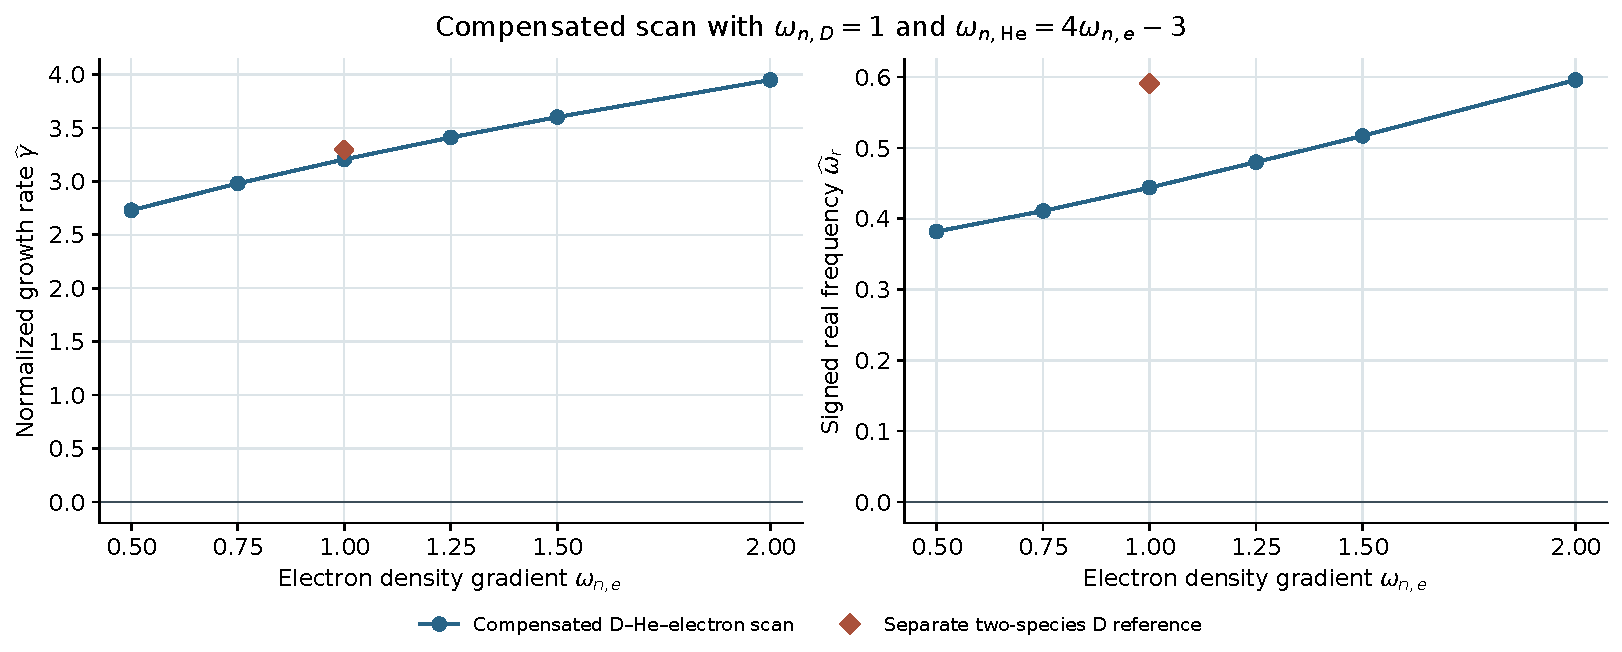
\includegraphics[width=\linewidth]{Figures/B_01_growth_and_signed_frequency.pdf}
\caption{GENE IV growth and signed frequency along the compensated path. The separate two-species deuterium control is marked at electron gradient 1. Contributor: Santos.}
\label{fig:additional-compensated-rates}
\end{figure}
